%\linenumbers*

%\chapter{FURTHER INVESTIGATIONS TO BUILD FUTURE RAINFALL INTENSITY SCENARIOS}
%\label{sec:FurtherInvestigationstoBuildFutureRainfallIntensityScenarios}

%\section{Proposed Simulation Methods}
\section{Possible Approaches to Simulating Future Rainfall Intensity}
\label{sec:ProposedSimulationMethods}

Despite the various efforts to find meaningful rainfall intensity trend for
building future scenarios of rainfall intensity changes, no significant trend
can be determined from analysing observed rainfall data in the study area.
Yet future rainfall intensities are predicted to increase.
%References and discuss why you did not find a trend (find it in CH3??)
However, even if the trend in rainfall intensity is available (for
example from an RCM), the results from this study indicate that knowing future
WSIV, WSIP and WSG is vital in order to carry out future erosion predictions. To
achieve the aim of this research, an alternative approach has to be sought to
obtain future rainfall data with a appropriate data resolution and
`changed' rainfall
intensity. The process of finding alternative approach is discussed in this
section.

%In order to predict changes of future rainfall intensity that are useful for
%estimating future soil erosion rates, it is vital to know how WSIV, WSG and
%WSIP are like in the future. However, even if we know these precisely for
%future, current models are not capable of utilising these properly because of
%the defects found previously (Section
%\ref{sec:EFFECTSOFCONTINOUSANDDISCONTINUSSTORM}).

%Thus, it has been suggested to analyse observed rainfall data to estimate a
%trend of rainfall intensity changes looking at a range of data scales. Based on
%the trend found, scenarios of future rainfall intensity were created.

%The analysis methods and the outcomes in this chapter are only presented to
%highlight limitations in our abilities to estimate future soil erosion rates.
%How future soil erosion may be estimated more adequately is also discussed in
%the latter section of this chapter.

%WEPP is used for the estimation of future soil erosion because only WEPP can
%perform continuous long term simulations.

\subsection{Approach 1: Changing CLIGEN Generated Data}
\label{sec:MethodOne}

%A similar method has been used in Section
%\ref{sec:MethodsSensitivityOfCLIGENToRainfallIntensityChanges}.
Daily peak rainfall intensity is changed by changing daily rainfall duration.
In a CLIGEN output, $R$, $D$, $t_p$ and $i_p$ comprise daily rainfall. These
are:
\begin{itemize*}
  \item $R$ : amount (inch)
  \item $D$ : duration (minute)
  \item $t_p$ : time to peak (normalised)
  \item $i_p$ : peak intensity (normalised)
\end{itemize*}
Among these four factors, duration ($D$) will be adjusted proportionally,
keeping other factors such as $t_p$, $i_p$ and $R$ constant. In this way, the
rainfall amount is kept constant, and rainfall intensity is varied.

Thirty year-long climate data were generated using CLIGEN with an input file,
which was prepared from the Southover dataset. Daily rainfall durations in this
30 year-long climate data were adjusted proportionally to obtain increased or
decreased daily peak rainfall intensities. Using the original and adjusted
climate data, runoff and soil erosion were to be simulated for 30 years. The
effect of \textit{indirect} rainfall intensity changes on runoff and erosion
were then analysed.

\paragraph{Pros:}
\label{sec:ProsMethodOne}
Simple, easy and fast.
%need more better justification
\paragraph{Cons:}
\label{sec:ConsMethodOne}
It may be considered to be crude and simple for simulating future rainfall
intensity changes. One reason is that it is not possible to change the number
of raindays using this approach. It does not make a full use of the findings
from the previous analyses. This is an indirect approach.

\subsection{Approach 2: Changing {MX.5P}, One of CLIGEN Input
Parameters}
\label{sec:MethodTwo}

\paragraph{Description of {MX.5P} (Yu, personal communication 2003)}
\label{sec:MX5PByBYu}

{MX.5P} is defined as ``Average maximum 30-min peak intensity (in/hr) for each
month''. If the sub-daily interval is denoted as $\Delta t$ (min), then there
are 1440/$\Delta t$ intervals, called $M_t$, in a day. For each wet day, discard
all the dry intervals to create a single storm event with \emph{continuous} rain
for, say, $M$ intervals. Then the storm duration, $D$, (min) is given by:
\begin{eqnarray}
  D = M \Delta t \delta
\end{eqnarray}

Find the maximum precipitation intensity for any 30-min period within the storm,
and call this $I_{30}$. If there are $n$ wet days in a month, find the maximum
of these $n$ $I_{30}$ values, and denote this maximum $I_{30}$ for the month as
$maxI_{30}$. If there are $K$ months on record, then {MX.5P} is given by:
\begin{eqnarray}
  \mathrm{MX.5P} = \frac{1}{K} \sum maxI_{30}
\end{eqnarray}

For example, let us say it rained on 3rd and 10th of May, 2001 with a peak
30-min intensity of 1.2 in/hr and 1.5 in/hr, respectively. Then $maxI_{30}$
would be 1.5 in/hr for May 2001. If we have 5 years of data for May:

\begin{table}[hbpt]
  \centering
  \begin{tabular}{ccc}
    \toprule
    Month & Year & $maxI_{30}$ (in/hr)\\
    \midrule
    May & 1997 & 0.8\\
    May & 1998 & 0.9\\
    May & 1999 & 0.3\\
    May & 2000 & 2.8\\
    May & 2001 & 1.5\\
    \bottomrule
  \end{tabular}
\end{table}

Then the {MX.5P} value for May for this hypothetical site would be:
\begin{equation}
  \frac{0.8+0.9+0.3+2.8+1.5}{5} = 1.26 \ \textrm{(in/hr)}.
\end{equation}

\paragraph{Changing {MX.5P}} The CLIGEN \emph{input} file was adjusted
accordingly rather than the CLIGEN
\textit{output} file. Two CLIGEN input files were prepared as if they are from
two different periods---present and future---of the site. Future climate changes
are thus conceptualised here as ``two different climate conditions in the same
place''. The original input file was built using observed event rainfall data
from Ditchling Road station. Rainfall intensity parameter ({MX.5P}) of the
original input file was adjusted accordingly to represent future rainfall
intensity changes (Table \ref{tab:MX5PChanges}). Two sets of CLIGEN-generated
weather data using these two input files only differ in peak rainfall
intensities, which is controlled by {MX.5P}. Then, WEPP simulates runoff and
soil
loss rates using these two CLIGEN climate data.

\begin{table}[htpb]
  \figureversion{tabular}
  \centering
  \caption{Ratio of {MX.5P} changes for each month}
  \label{tab:MX5PChanges}
    \begin{tabular}{lcccc}
    \toprule
    & \multicolumn{2}{c}{Decrease} & \multicolumn{2}{c}{Increase} \\
    \cmidrule(r){2-3} \cmidrule(l){4-5}
    Wet Season (SONDJF months)   & $-$10\% &  $-$5\%  & $+$5\%  & $+$10\% \\
    Dry Season (MAMJJA months)   & $-$10\%  & $-$5\%  & $+$5\%  & $+$10\% \\
    \bottomrule
    \end{tabular}
\end{table}

Few studies pointed out that the ratio of wet and dry days will influence the
behaviour of future soil erosion
\citep{nearing2001-229,pruski2002-climate,pruski2002-7}. However, as this thesis
only concentrates on the implication of rainfall intensity changes, no rainfall
frequency change is considered. No rainfall amount change is also assumed here.
Due to the lack of information, no intra-storm rainfall intensity pattern for
the future was considered.

Nearing (personal e-mail communications, 8 June 2001) pointed out that, if
MEAN~P in CLIGEN input file is changed together with {MX.5P}, we would end up
with completely different climate data from what we have started with. Also,
generated data may not have clear relationships with original data. This is a
problem for a sensitivity-type comparison---that is, comparing how WEPP
estimates differ for two well-defined sets of input data. On the other hand,
when creating ``realistic'' future rainfall data is to be the main concern, both
parameters (MEAN~P and {MX.5P}), together with other parameters may need to be
changed. It will, however, only be applicable to the case where sufficient
reference data are available for the adjustment and comparison of all the
parameter. No such information has been available for this research. Therefore,
until such information is available, it is important to limit the changes only
to a single parameter, {MX.5P} in this case, and carry out only the
sensitivity-type comparison.

It is very unlikely all the months will have the same changes in rainfall
intensity. There will be some degrees of variations depending on seasons, for
example. Two seasonal variations are considered here---Wet and Dry season. The
wet season includes September, October, November, December, January and February
(Table \ref{tab:AdjustedMX5Pvaluesforwetseasons}). The dry season consists of
March, April, May, June, July and August (Table
\ref{tab:AdjustedMX5Pvaluesfordryseasons}).

\begin{table}[htbp]
  \figureversion{tabular}
  \centering
  \footnotesize
  \caption{Adjusted {MX.5P} values for the wet season}
  \label{tab:AdjustedMX5Pvaluesforwetseasons}
    \begin{tabular}{r|cc|cccccc|cccc}
      \toprule
      month & \textbf{1} & \textbf{2} & 3 & 4 &5& 6& 7& 8& \textbf{9}
&\textbf{10}& \textbf{11}& \textbf{12}\\
      \midrule
      $-$10\% & 0.24 & 0.16 & 0.23 & 0.23&  0.27 & 0.33 & 0.42 & 0.58 & 0.39 &
0.41 & 0.31 & 0.27\\
      $-$5\%  &0.26 & 0.17 & 0.23 & 0.23 & 0.27 & 0.33 & 0.42 & 0.58 & 0.41 &
0.43 & 0.32 & 0.28\\
      original & 0.27 & 0.18 & 0.23  &0.23 & 0.27 & 0.33 &0.42 & 0.58 & 0.43 &
0.45 & 0.34 & 0.30\\
      5\% & 0.28 & 0.19 & 0.23 & 0.23 & 0.27 & 0.33 & 0.42& 0.58 & 0.45 & 0.47 &
0.36 & 0.32\\
      10\% & 0.30 & 0.20 & 0.23 & 0.23 & 0.27 & 0.33 & 0.42 & 0.58 & 0.47& 0.50
& 0.37 & 0.33\\
      \bottomrule
    \end{tabular}
\end{table}

\begin{table}[htbp]
  \figureversion{tabular}
  \centering
  \footnotesize
  \caption{Adjusted {MX.5P} values for the dry season}
  \label{tab:AdjustedMX5Pvaluesfordryseasons}
    \begin{tabular}{r|cc|cccccc|cccc}
      \toprule
      month & 1 &2& \textbf{3} &\textbf{4} &\textbf{5}& \textbf{6}& \textbf{7}&
\textbf{8}& 9 &10& 11& 12\\
      \midrule
      $-$10\%  &0.27&  0.18  &0.21 & 0.21 & 0.24 & 0.30 & 0.38 & 0.52 & 0.43 &
0.45 & 0.34&  0.30\\
      $-$5\% & 0.27 & 0.18 & 0.22  &0.22  &0.26  &0.31 & 0.40& 0.55 & 0.43 &
0.45 & 0.34 & 0.30\\
      original&  0.27  &0.18 & 0.23  &0.23 & 0.27 & 0.33 &0.42  &0.58 & 0.43&
0.45 & 0.34 & 0.30\\
      5\%  &0.27 & 0.18&  0.24& 0.24 & 0.28 & 0.35 & 0.44 &0.61 & 0.43 & 0.45 &
0.34 & 0.30\\
      10\% & 0.27  &0.18 & 0.25  &0.25  &0.30  &0.36 & 0.46& 0.64 & 0.43 &0.45
&0.34  &0.30 \\
      \bottomrule
    \end{tabular}
\end{table}

Since soil erosion is closely related to the extreme rainfall events, this
thesis concentrates on extreme rainfall events which are closely related to the
rainfall parameter, {MX.5P}. This is the main reason why {MX.5P} is chosen to be
altered. It is clear that \citet{nicks1995-2} has recognised the close
statistical relationship between {MX.5P} and soil erosion rate. Thus, it is
unsurprising that this parameter is explicitly included in the CLIGEN input
file.

\paragraph{Pros:}
\label{sec:ProsMethodTwo}
The procedures are relatively easy and uncomplicated. Calculating {MX.5P} is
relatively straightforward from tipping-bucket data. It does change the rainfall
intensity of extreme events.

\paragraph{Cons:}
\label{sec:ConsMethodTwo}
Generated rainfall data for the original and ``future'' climate are almost the
same except for rainfall intensity. Thus the ``future condition'' here is not,
physically, very realistic. Future climate will change in complex ways, not
only extreme rainfall intensity will change, but also probabilities of raindays,
WSIP (Within-Storm Intensity Pattern) and rainfall amount will very
probably also change.
Also, even if we increase or decrease extreme rainfall intensity only, the
intensity of small rainfall events are also affected in order to keep overall
annual rainfall amount constant.

\subsection{Approach 3: Using GCM/RCM Data}
\label{sec:MethodThree}

This third approach described here was proposed originally, but has not been
used
because there were no GCM data which were suitable for this research because of
the scale mismatch.
% (see Chapter \ref{sec:LimitationsOfErosionModels}) -- is this relevant?.
Nevertheless, daily RCM data for current and future climate have been acquired.
RCM also produced 20-min rainfall data, but with a high variability. Daily
rainfall intensity (or amount) is not suitable to be used as erosion model input
directly unless downscaled.

The procedures of this approach are:
\begin{enumerate*}
  \item GCM data with 30-min time step for current and future climate
  \item CLIGEN input files for current and future climate are built
  \item CLIGEN generates climate data for current and future climate
  \item WEPP simulates runoff and erosion for current and future climate.
\end{enumerate*}

It might be possible to calculate all the CLIGEN input parameters out of the GCM
output. GCMs can generate current and future climate data on a
sufficient temporal
resolution---that is, 30-min time step---for building CLIGEN input files.
This will permit a ``better''---in the sense of being more realistic---judgement
of impacts of rainfall intensity changes on future soil erosion.

%There are some possible caveats with this approach.
%One is that these high-resolution model-generated GCM data may have
%problems and errors caused by unconventional configurations on the top of GCMs'
%uncertainty and wide range of variations.
A major caveat is that the high resolution GCM data are still not readily
available. A separate model configuration is required to generate this
kind of data, and the set-up process usually requires extended model set-up
skills and simulation times. This was the case for the current research.
Another possible problem is that, because of the preceding uncertainty of GCM
output, we might end up with erroneous CLIGEN input files which, in turn, will
lead to even greater errors for future erosion estimation.

%summary table here

\subsection{Conclusion: Selected Approach}
\label{sec:SelectedMethod}

Approach 2 (Section \ref{sec:MethodTwo}) is selected. The schematic
procedure of this approach is shown in Figure
\ref{fig:future_erosion_flowchart}.
It was assumed that future WSIV, WSG and WSIP are the same as the present. Only
monthly maximum of 30-min peak rainfall intensity was considered for
constructing future rainfall intensity scenarios.

CLIGEN generates original climate data using the input file which statistically
represents the characteristics of current rainfall intensity. Keeping all other
parameters constant, the intensity parameter ({MX.5P}) in the CLIGEN input file
are increased or decreased proportionally (Table \ref{tab:MX5PChanges}).
{MX.5P} is specifically related to extreme intensity events as given by its
definition, `Average maximum 30 minutes peak intensity (in/hr) for each month'.
``Future'' climate data are then generated using adjusted CLIGEN input file.
WEPP simulates runoff and soil loss using both climate data. Runoff and soil
loss changes are compared with changes in rainfall intensity.

\begin{figure}[htpb]
  \centering
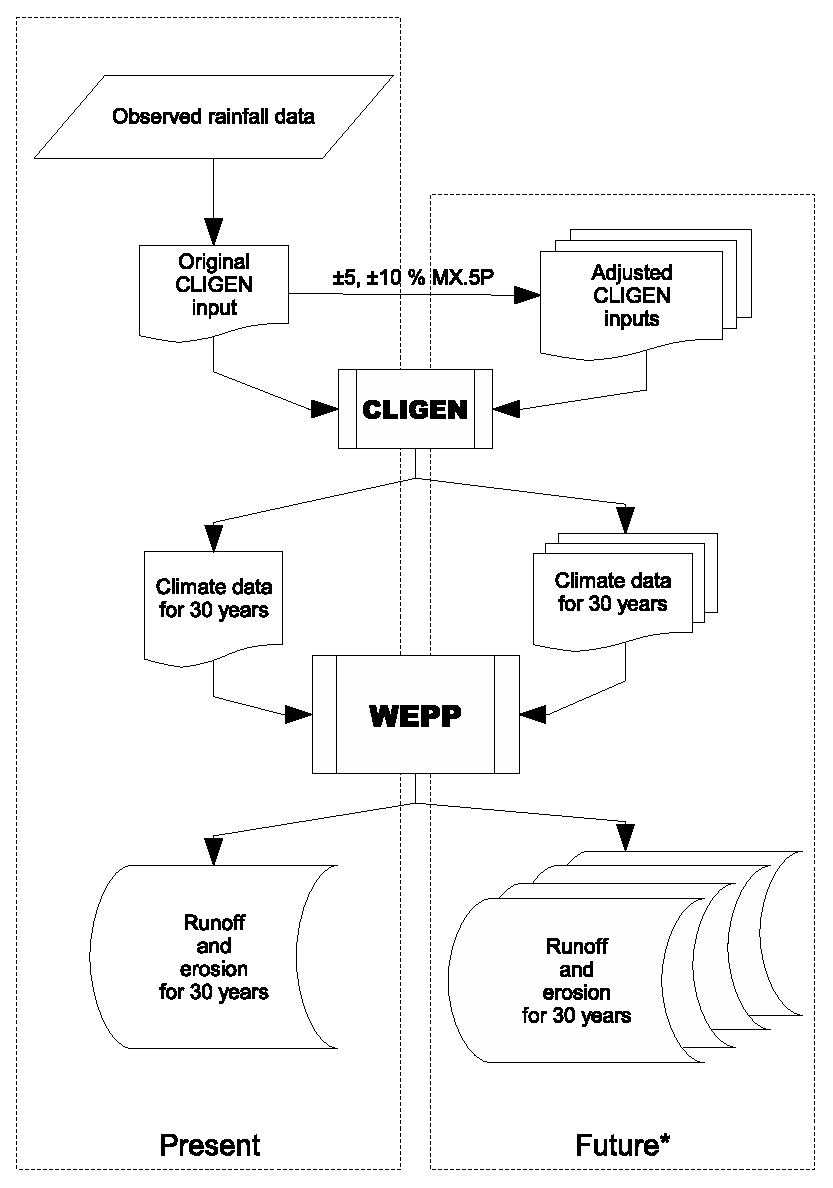
\includegraphics[width=0.8\textwidth]{./img/future_erosion_flowchart}
  \caption[Schematic flowchart of the approach used for investigation of
implications of rainfall intensity changes for future soil erosion]{Schematic
flowchart of the approach which is used for investigation of implications of
rainfall intensity changes for future soil erosion. Soil erosion simulated in
the left-side box marked with `Present' represents the present erosion rate
under current rainfall intensity. Soil erosion simulated in the right-side box
marked with `Future*' represents assumed future erosion rates under the
different rainfall intensities.}
  \label{fig:future_erosion_flowchart}
\end{figure}

%\nolinenumbers
